\documentclass[conference]{IEEEtran}
\usepackage[T1]{fontenc}
\usepackage{newtxtext,newtxmath,graphicx,booktabs,tabularx,array,amsmath,microtype}
\usepackage[table]{xcolor}
\usepackage[colorlinks=true,urlcolor=blue!55!black,citecolor=teal!65!black,linkcolor=teal!65!black]{hyperref}
\definecolor{RRlight}{HTML}{EAF5F5}
\graphicspath{{figures/}}
\newcommand{\fig}[3]{\begin{figure}[!t]\centering\includegraphics[width=\columnwidth]{#1}\caption{#2}\label{#3}\end{figure}}
\title{Reading the Reading Room: A Reproducible Study of Lung-Focused CNN--Transformer Pneumonia Classification}
\author{\IEEEauthorblockN{Samarth Shekhar}\IEEEauthorblockA{230042\\Computer Vision Project}\and\IEEEauthorblockN{Meghavi Rao}\IEEEauthorblockA{230044\\Computer Vision Project}\and\IEEEauthorblockN{Rachit Kumar}\IEEEauthorblockA{230128\\Computer Vision Project}\and\IEEEauthorblockN{Harshal Nerpagar}\IEEEauthorblockA{230076\\Computer Vision Project}}
\begin{document}\maketitle
\begin{abstract}
We document a complete student research workflow for normal-versus-pneumonia classification on pediatric chest radiographs: literature selection, three baseline reconstructions, a pre-implementation hypothesis, controlled anatomical cropping and transformer comparisons, and an auditable demonstration. Initial cached five-epoch accuracy was 87.18\%; a 15-epoch cached audit achieved 85.74\%; a corrected five-epoch online ensemble achieved 92.15\%. Our final resource-bounded pilot freezes ImageNet-pretrained ResNet18 and DeiT-Tiny encoders and trains four classifier heads for five epochs. Fixed pretrained segmentation supplies lung-focused crops from original-resolution pixels. On 624 benchmark test records, the crop-plus-transformer condition achieves 93.75\% accuracy, 98.21\% pneumonia sensitivity, 86.32\% specificity, macro F1 0.9318 and AUC 0.9757. The paired crop-only macro-F1 difference is +0.0696, with proxy-group bootstrap 95\% interval [0.0404, 0.1016]. However, cropping reduces validation performance while improving test performance. We therefore report a split-dependent benchmark result, with explicit scope reductions, preserved failures and verification, rather than a clinical or state-of-the-art claim. Code, model weights, predictions, source manifests and presenter materials accompany the report.
\end{abstract}
\begin{IEEEkeywords}Chest X-ray, pneumonia, transfer learning, lung cropping, vision transformer, reproducibility, failure analysis.\end{IEEEkeywords}

\section{Introduction and Project Objectives}
Public chest X-ray benchmarks allow students to build and inspect computer vision systems with limited resources. A high score alone does not explain which design choice helped, whether the score repeats, or whether the software actually runs from its saved artifacts. We therefore study both the numerical result and its reproducibility.

Our milestones are: M1, review prior work; M2, reconstruct a working baseline; M3, record a numerical hypothesis before implementation; M4, implement and compare controlled conditions; M5, analyze failures and deliver the report, demonstration and defence. The original direction was InceptionV3 on the Kermany collection. We changed the reference to the five-CNN approach of Chouhan \emph{et al.}~\cite{chouhan}, while retaining lung cropping as the primary proposed intervention. A pretrained transformer was added as a separately tested extension.

The project contributions are a transparent reconstruction history, a controlled four-condition pilot, and an executable path from saved weights to the interface. Lung cropping and CNN--transformer combinations are existing ideas~\cite{hybrid,deit}; we do not claim a globally new architecture. The final experiment is deliberately smaller than the original proposal and is identified accordingly throughout.

\section{Literature Review and Source Corrections}
The M1 survey reviewed the nine lines of work in Table~\ref{tab:lit}. Dataset papers motivated transfer learning; compact CNN comparisons motivated feasible backbones; ensemble and transformer studies motivated complementary predictors. These were reviewed as background, not all independently reproduced.
\begin{table}[!t]\caption{M1 literature lineage and project relevance.}\label{tab:lit}\centering\footnotesize\begin{tabularx}{\columnwidth}{@{}lX@{}}\toprule\rowcolor{RRlight}Work & Role\\\midrule
Kermany, 2018 & Pediatric dataset and transfer learning.\\
CheXNet, 2017 & DenseNet chest-radiograph classification.\\
Wang, 2017 & Large datasets and localization benchmarks.\\
Stephen, 2019 & Compact CNN trained from scratch.\\
Ayan and Unver, 2019 & Backbone comparison and ensembles.\\
Rahman, 2020 & Pretrained backbone comparisons.\\
Chouhan, 2020 & Selected five-CNN reconstruction target.\\
Rajaraman, 2018 & Activation-map interpretation.\\
Singh, 2024 & Larger pretrained transformer context.\\\bottomrule\end{tabularx}\end{table}

Chouhan \emph{et al.} combine AlexNet, DenseNet121, InceptionV3, GoogLeNet and ResNet18 by majority voting~\cite{chouhan}. Their reported accuracy is 96.39\%, sensitivity 99.62\%, precision 93.28\% and AUC 0.9934, with schedules of 50--200 epochs. Our CPU experiments use shorter schedules and documented assumptions because exact author settings, manifests or paper-linked source code were not recovered. A generic student implementation is not treated as author code.

The source audit corrected over-broad M1 claims that all papers used the same 624 test cases or omitted F1 and confidence intervals. The transformer comparison uses a different split and reports additional metrics. We also withdrew the idea that overlap of separate intervals establishes statistical equivalence, and the assumption that a bounding crop removes every shortcut. The archived M1 deck is historical; this corrected account takes precedence.

Later work reports higher numerical results, including HybridCATNet's 96.93\% under harmonized-data cross-validation~\cite{hybrid}, and an AutoML study's 98.6\% under a different image-level internal split~\cite{automl}. The latter acknowledges uncertain patient independence and absent external validation. These reported scores do not form a common industry leaderboard against our model.

\section{Data, Partitions and Measurement}
\subsection{Verified source preparation}
We use the public pediatric collection associated with Kermany \emph{et al.}~\cite{data}, through the recorded Hugging Face mirror. Original counts are 5,216 training, 16 validation and 624 test records. The paper-style baseline merges training and original validation into 5,232 records: 1,349 normal and 3,883 pneumonia.

The audited and final-pilot protocol yields 5,206 deduplicated non-test records, with 4,164 training and 1,042 validation cases. The original 624 test records remain intact for comparison; they contain 234 normal and 390 pneumonia labels. Unique-image sensitivity analysis uses 618 test images. The complete final preprocessing workload contains 5,824 unique source images.

Source parquet hashes are checked before extraction. Each final full-image resize from original source pixels was also checked against the earlier 224-pixel cache. Only one source shard is processed at a time. This controls disk consumption while allowing crops to be taken before classification resizing.
\begin{table}[!t]\caption{Final-pilot partitions.}\label{tab:split}\centering\begin{tabular}{lrrr}\toprule\rowcolor{RRlight}Partition & Normal & Pneumonia & Total\\\midrule
Training & 1,078 & 3,086 & 4,164\\
Validation & 270 & 772 & 1,042\\
Test records & 234 & 390 & 624\\\bottomrule\end{tabular}\end{table}

\subsection{Grouping and evaluation boundaries}
Pneumonia person numbers, normal filename prefixes and hashes supply conservative grouping proxies. They do not independently verify patient identity. The test set was inspected in earlier project experiments and is not a blind external holdout. Single-center pediatric data also cannot establish performance across institutions, adult cohorts, devices or clinical differentials.

For pneumonia as the positive class, sensitivity is $TP/(TP+FN)$, specificity $TN/(TN+FP)$ and precision $TP/(TP+FP)$. Both class F1 scores are reported, with their unweighted mean as macro F1. Accuracy and confusion matrices use fixed decisions; AUC uses continuous scores. AUC measures ranking, not calibration.

The crop-only comparison uses 1,000 paired resamples of the same test cases under conservative filename-group proxies. This interval describes the benchmark conditional on that grouping approximation. It does not include independently trained seed variation, alternative partitions or external cohorts. Duplicate-image sensitivity analysis is reported separately.

\section{M2: Three Main Baseline Experiments}
\subsection{Preliminary diagnostics}
Small head-only probes and partial resumable feature caches preceded the headline baseline. Their files are retained as diagnostics, not presented as additional completed five-model experiments. Inspecting the paper's architecture clarified that a classifier-only probe differs from training the specified late CNN blocks.

\subsection{Initial cached five-epoch run}
To reduce compute, we stored frozen-prefix activations and trained late blocks or replacement classifiers using a clean and one fixed seeded augmented view. Reduced-precision stored activations were converted back for training. The five-model majority vote reached 87.18\% accuracy, 99.74\% sensitivity, 66.24\% specificity and macro F1 0.8508. Its confusion matrix contained 79 false positives and one false negative. High pneumonia recall therefore concealed weak normal-case recognition.

\subsection{Fifteen-epoch cached audit}
The second run used the group-aware split and four fixed views. Validation selected epochs 13, 9, 5, 13 and 1 for ResNet18, DenseNet121, GoogLeNet, InceptionV3 and AlexNet, respectively. Selected validation ensemble accuracy was 98.94\%, but test accuracy was 85.74\%, specificity 62.39\% and macro F1 0.8319, with 88 false positives and one false negative.

Independent checks did not find a stale-feature, label-order or metric-arithmetic explanation sufficient to resolve that validation/test gap. The cause remained unresolved. This comparison changes split, views and checkpoint selection as well as duration, so it cannot demonstrate that more epochs inherently hurt performance.

\subsection{Corrected online five-epoch reconstruction}
The third run restored all 5,232 paper-training records, complete FP32 forwards and fresh augmentation. Early weights remained fixed while BatchNorm running statistics adapted. Fresh flips, resized crops, intensity variation and shared grayscale noise replaced the finite-view approximation. Final epoch-five checkpoints were fixed in advance. Three models trained on the Mac and two in the isolated CPU VPS.

Accuracy rose to 92.15\%, sensitivity was 94.62\%, specificity 88.03\%, macro F1 0.9157 and AUC 0.9623. There were 28 false positives and 21 false negatives. ResNet18 alone reached 93.11\% accuracy, illustrating that additional models do not automatically improve the chosen aggregation rule. This is the final M2 baseline; older results remain preserved.
\begin{table*}[!t]\caption{Historical experiments. Multiple settings change between rows; these are descriptive results, not an epoch-only or crop-only ablation.}\label{tab:history}\centering\small\begin{tabular}{lrrrrrr}\toprule\rowcolor{RRlight}Experiment & Accuracy & Sensitivity & Specificity & Precision & Macro F1 & AUC\\\midrule
Cached five epochs & 87.18\% & 99.74\% & 66.24\% & 83.12\% & 0.8508 & 0.9815\\
Cached fifteen-epoch audit & 85.74\% & 99.74\% & 62.39\% & 81.55\% & 0.8319 & 0.9723\\
Corrected online five epochs & 92.15\% & 94.62\% & 88.03\% & 92.95\% & 0.9157 & 0.9623\\
Earlier online ResNet18 component & 93.11\% & 95.38\% & 89.32\% & 93.70\% & 0.9260 & 0.9733\\
Final crop CNN--ViT pilot & 93.75\% & 98.21\% & 86.32\% & 92.29\% & 0.9318 & 0.9757\\\bottomrule\end{tabular}\end{table*}
\begin{figure*}[!t]\centering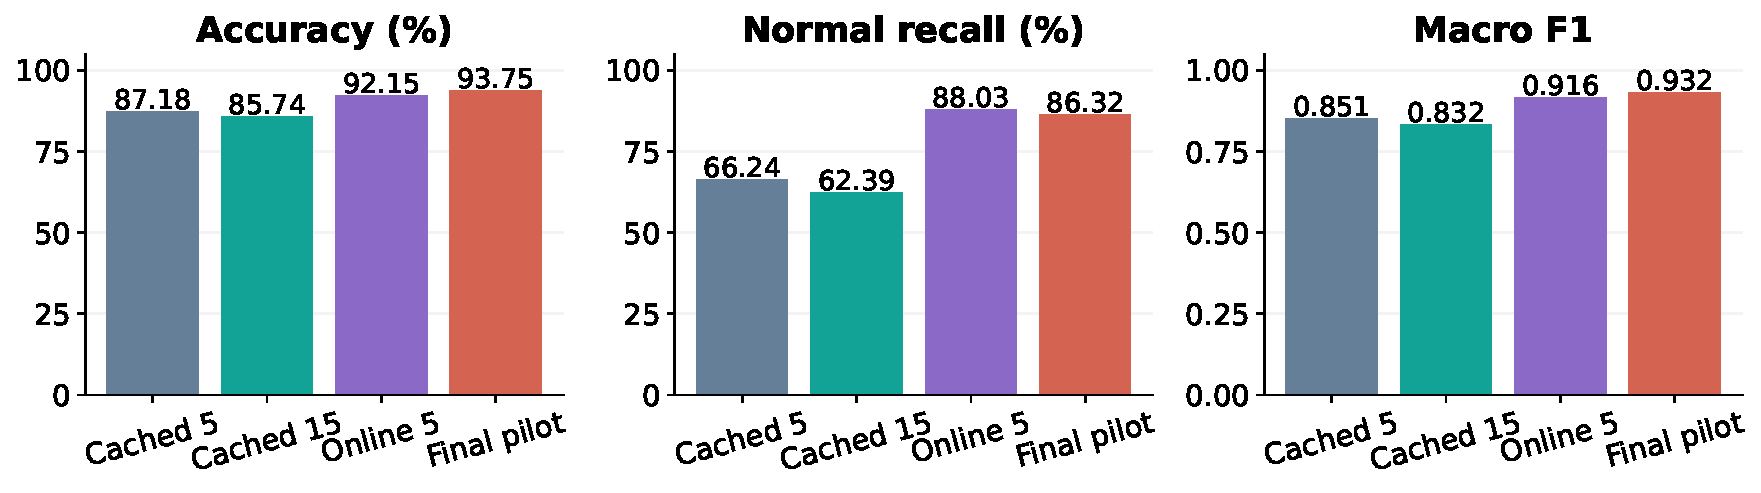
\includegraphics[width=\textwidth]{history.pdf}\caption{The historical progression is non-monotonic. It motivated implementation auditing rather than selecting a flattering score. Differences across protocols cannot isolate one cause.}\label{fig:history}\end{figure*}

\section{M3: Hypothesis Before Implementation}
The 5 October 2026 revision proposed cropping as the primary intervention and a small pretrained transformer as a separate extension. For crop-only comparison, predicted macro F1 improvement was 0.01--0.03, specificity improvement 2--5 percentage points and AUC improvement 0.00--0.02. Pneumonia recall was predicted to remain within two points of the control. The combined proposal predicted macro F1 +0.01--0.04 and accuracy 0--3 points, with recall loss no greater than two points.

These ranges are preserved predictions, not edited to match the observed gains. They superseded earlier tentative M1 expectations. The measured test changes exceed the predicted magnitude, while the validation reversal below limits broader interpretation.

\section{M4: Final Controlled Pilot}
\subsection{Explicit scope reduction}
The original extension retained all five CNNs. Our final compute-bounded pilot substitutes a single ResNet18 and freezes both encoders, optimizing linear heads only. It is a reduced experiment, not the complete original five-CNN crop ablation, a full-schedule paper reproduction, or a reproduction of the larger DeiT-Base paper. M2's online experiment remains separate. No fresh augmentation is used in the final frozen-feature pilot; M2 already implemented fresh augmentation.

\subsection{Anatomical cropping}
Fixed TorchXRayVision ChestX-Det PSPNet supplies left- and right-lung channels~\cite{xrv}. Grayscale pixels use the library normalization and model transform. Sigmoid outputs are thresholded at 0.5, and the lung union defines a bounding rectangle with 10\% margin per side. Coordinates map back to original RGB pixels before the $224\times224$ classification resize.

The official wrapper uses 512 pixels. A runtime pilot measured about 3.72 seconds per image there, versus approximately 0.84 seconds at 256. We used the same underlying pretrained model at 256 pixels, documenting that departure. All final masks are uniform 256; initial 512 outputs were recomputed. Resolution was selected for runtime, without using test classification outcomes.

Empty masks or area fractions below 0.08 or above 0.85 trigger full-image fallback. Passing these checks does not prove anatomical correctness. A bounding rectangle retains some heart, markers or peripheral information. No manual masks support a segmentation IoU claim.
\fig{segmentation_pipeline.png}{Actual training example: full resize, predicted mask and crop from original-resolution source pixels. The mask is a model prediction, not manual ground truth.}{fig:pipeline}

\subsection{Encoders, heads and aggregation}
Fixed ImageNet ResNet18 and DeiT-Tiny encoders~\cite{deit} produce 512- and 192-dimensional representations. Full/crop variants have separate linear two-class heads. Training-only feature means and standard deviations are used, with a 0.001 standard-deviation floor. AdamW uses learning rate 0.001, weight decay 0.01, batch size 32, unweighted cross-entropy, seed 42, FP32 and two CPU threads for five epochs. Validation macro F1 chooses checkpoints, with earlier epochs breaking ties; all selected epoch five.

The four conditions in Table~\ref{tab:conditions} separate region and aggregation. For pneumonia probabilities $p_R$ and $p_V$,
\begin{equation}p_{blend}=(1-w)p_R+wp_V.\end{equation}
Validation evaluates $w\in\{0,0.25,0.5,0.75,1\}$, retaining the earlier lower weight on ties. C selects $w=0.25$ and D $w=0.50$. Labels use a fixed 0.5 threshold. D is the predeclared target, not a winner selected across conditions after observing test scores.
\begin{table}[!t]\caption{Matched final conditions.}\label{tab:conditions}\centering\footnotesize\begin{tabularx}{\columnwidth}{@{}clX@{}}\toprule\rowcolor{RRlight}Run & Input & Decision\\\midrule
A & Full & ResNet18 head\\B & Crop & ResNet18 head\\C & Full & $0.75p_R+0.25p_V$\\D & Crop & $0.50p_R+0.50p_V$\\\bottomrule\end{tabularx}\end{table}

\section{Results and Interpretation}
\subsection{Matched test effects}
Cropping alone raises accuracy from 86.86\% to 92.63\% and macro F1 from 0.8503 to 0.9199 (Table~\ref{tab:results}). Specificity increases 16.67 points while sensitivity falls 0.77 points: 39 fewer false positives and three additional false negatives. The paired crop macro-F1 change is +0.0696, with proxy-group 95\% interval [0.0404, 0.1016]. It is evidence within this benchmark and grouping approximation.

Adding ViT to full images improves accuracy 1.28 points and macro F1 0.0153; adding it to crops improves accuracy 1.12 points and macro F1 0.0118. D makes six fewer false negatives and one fewer false positive than B. Combined D minus A is +6.89 accuracy points and +0.0814 macro F1. Effects were measured, not assumed additive.
\begin{table*}[!t]\caption{Final test metrics on 624 records. Confusion matrices use true Normal/Pneumonia rows and predicted Normal/Pneumonia columns.}\label{tab:results}\centering\small\begin{tabular}{crrrrrrl}\toprule\rowcolor{RRlight}Run & Accuracy & Sensitivity & Specificity & Precision & Macro F1 & AUC & Matrix\\\midrule
A & 86.86\% & 97.44\% & 69.23\% & 84.07\% & 0.8503 & 0.9308 & $[162,72;10,380]$\\
B & 92.63\% & 96.67\% & 85.90\% & 91.95\% & 0.9199 & 0.9703 & $[201,33;13,377]$\\
C & 88.14\% & 97.95\% & 71.79\% & 85.27\% & 0.8656 & 0.9472 & $[168,66;8,382]$\\
\rowcolor{RRlight}D & 93.75\% & 98.21\% & 86.32\% & 92.29\% & 0.9318 & 0.9757 & $[202,32;7,383]$\\\bottomrule\end{tabular}\end{table*}
\begin{figure*}[!t]\centering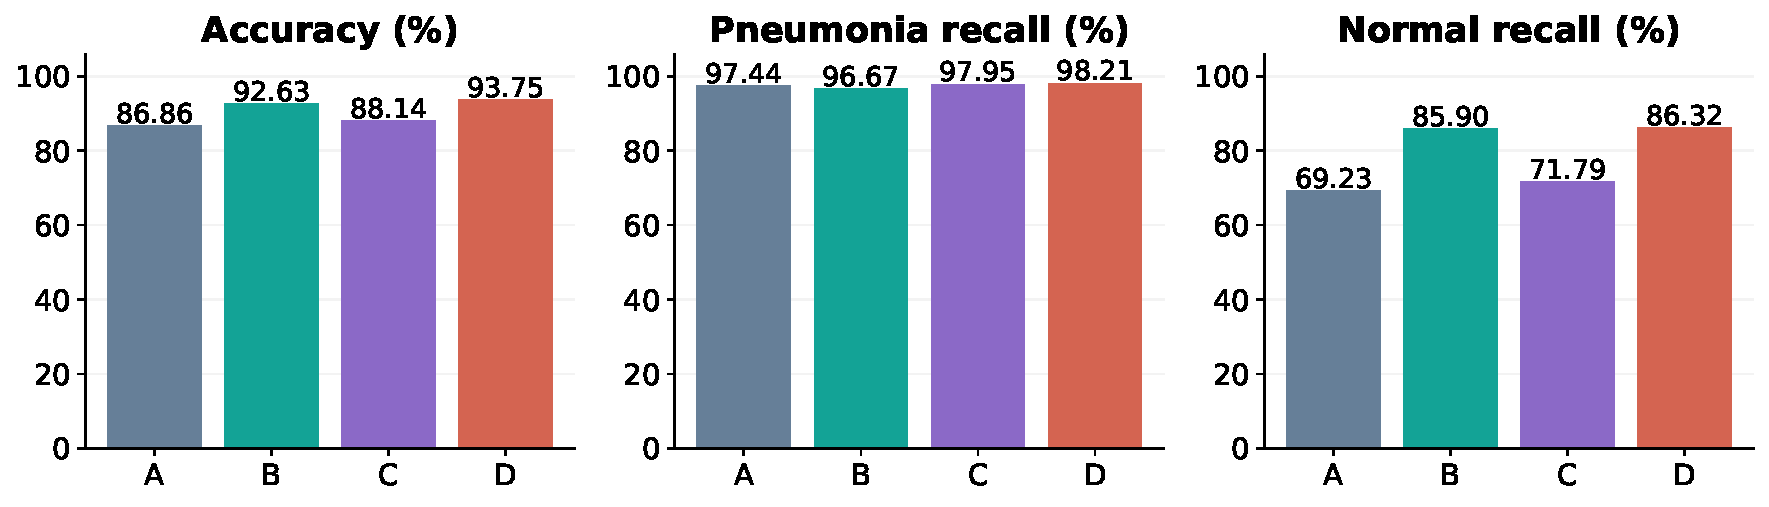
\includegraphics[width=\textwidth]{ablations.pdf}\caption{The four matched test comparisons. Cropping is the larger observed intervention; ViT adds smaller gains under both image conditions.}\label{fig:ablations}\end{figure*}
\fig{roc.pdf}{ROC curves computed from saved per-record probabilities. AUC is a ranking metric, not calibration.}{fig:roc}

\subsection{Validation/test reversal}
Validation macro F1 is A 0.9549, B 0.9072, C 0.9573 and D 0.9243. Cropping therefore \emph{reduces} validation performance while improving test performance (Fig.~\ref{fig:val}). Differences in composition or acquisition are possible explanations, but no cause is established from this one split. This prevents claims of universal crop superiority.

Validation still selects heads and mixture weights within each condition, and the independent audit recomputes that selection. D's target designation predates implementation. Repeated patient-aware partitions and external data are required to test stability.
\fig{validation_test.pdf}{The direction of cropping's effect reverses between validation and test. This is a material split-sensitivity result, not a resolved explanation.}{fig:val}
\begin{figure*}[!t]\centering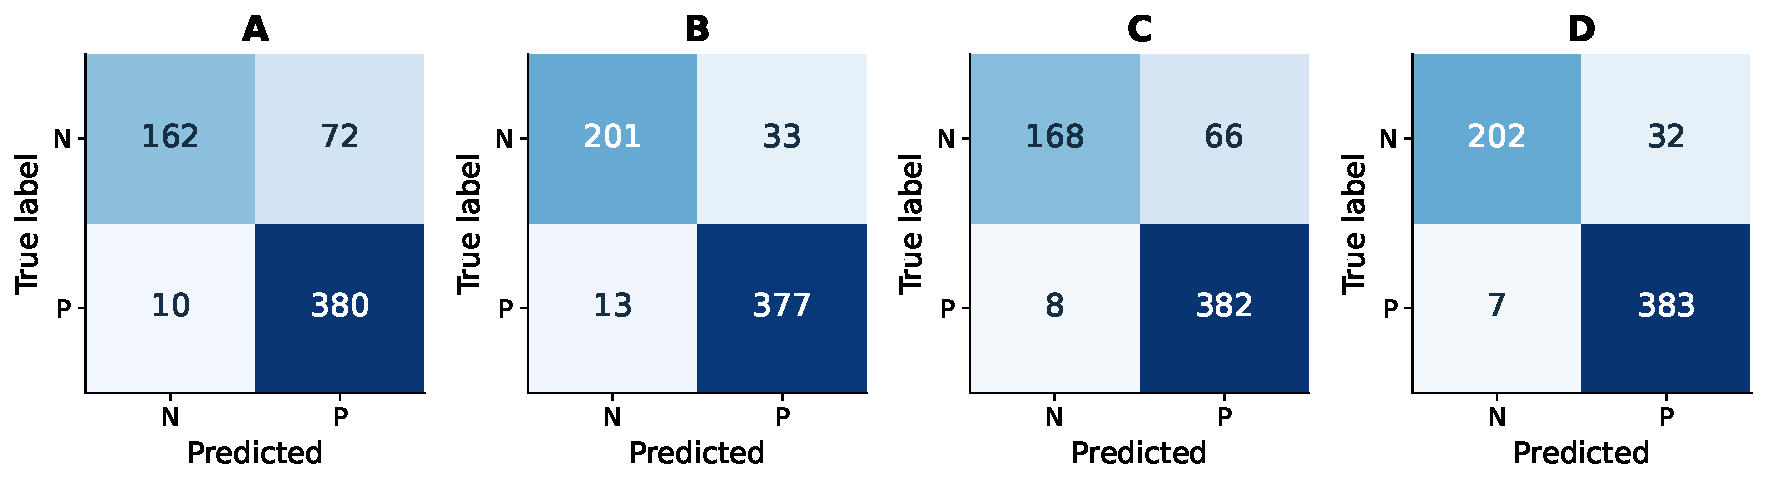
\includegraphics[width=\textwidth]{confusion.pdf}\caption{All test confusion matrices (N: normal; P: pneumonia). D finds 383 of 390 pneumonia records and correctly recognizes 202 of 234 normal records.}\label{fig:cm}\end{figure*}

\subsection{Historical and paper comparison}
D makes 39 rather than the corrected M2 ensemble's 49 errors. Missed pneumonia falls from 21 to seven, while false alarms rise from 28 to 32. Accuracy improves 1.60 points, sensitivity 3.59 points and macro F1 0.0160, while specificity falls 1.71 points. Against the old ResNet18 component, accuracy improves only 0.64 points, or four cases. The new model is not better on every metric.

Historical runs have different training partitions, boundaries and aggregation, so those differences cannot isolate cropping. A/B/C/D provide the controlled comparison. The base paper's reported accuracy remains 2.64 points higher than D, and its reported AUC is 0.9934 versus 0.9757. Training-budget and unknown-setting differences provide context, not a demonstrated causal explanation of the gap.

The 618-unique-image analysis gives D accuracy 93.69\%, sensitivity 98.19\%, specificity 86.15\%, macro F1 0.9310 and AUC 0.9755. Removing six repeated test images changes the headline result little, without establishing patient independence.

\section{M5: Failure and Resource Analysis}
\subsection{Mask and crop failures}
Automatic fallback occurs for 82/5,824 unique images (1.41\%). Median retained original area is 71.10\%, ranging 17.72--100\%; 100\% includes fallbacks. The record audit identifies training fallbacks of one normal and 63 pneumonia images, validation fallbacks of 11 pneumonia images, and test fallbacks of seven pneumonia records.

The illustrated automatic failures have too-small or partial-lung masks. The full-image fallback avoids applying those crops, but does not guarantee correct classification. Qualitative training examples were selected under a declared class-balanced policy, without changing thresholds to optimize test results. The automatic flag rate is not segmentation error rate.
\fig{crop_areas.pdf}{Distribution of retained original-image area. A rectangle changes input allocation but does not isolate exact lung pixels.}{fig:areas}
\fig{fallback_pipeline.png}{A training fallback: an implausibly small predicted mask causes the full image to be retained.}{fig:fallback}

\subsection{Classification and explanation limits}
D still misses seven pneumonia records and generates 32 false alarms. Eight selected errors are shown in the appendix. We can inspect scores, positioning and masks, but no lesion annotation or clinical adjudication establishes a medical explanation for an error.

The earlier research interface computes genuine ResNet18 Grad-CAM from corrected M2 weights. It explains that component's response to a displayed class, not the full ensemble or a verified pneumonia boundary. The final presenter interface shows original image, predicted anatomy, crop and the selected classifier output. Anatomical masks and class attributions are different quantities.

\subsection{Compute and implementation findings}
The final run uses an isolated two-core CPU workspace with a 6 GB memory allowance. The interval between first and last final mask files is 102.72 minutes, including pauses and later downloads but excluding initial weights and first-shard download. Feature passes take several minutes each; head optimization duration was not independently captured.

Resource guards paused without out-of-memory crashes. One guard underestimated reclaimable clean file cache and was corrected while retaining a 512 MB reserve. A separate transformer issue retained complete patch-token backing tensors behind NumPy class-token views. Copying the 192-dimensional vector removed memory growth without changing values or statistical settings. Cached crops and features enabled resumption. These corrections are not new classification treatments or test-driven selection.

The segmenter has 68,068,316 parameters; ResNet18 and DeiT-Tiny encoders have 11,176,512 and 5,524,416. CNN and ViT heads have 1,026 and 386 parameters each. D uses 84,770,656 neural-network parameters, with only 1,412 head parameters optimized for D. The fixed segmenter remains a substantial inference cost.

Server-side processing measured 1.24--1.49 seconds on two prepared samples and 4.58 seconds on an uploaded 224-pixel fixture: 3.52 seconds preprocessing and 1.03 seconds classifier processing. These include relevant loads and encoding and exclude HTTP transport. They are fixture measurements, not latency guarantees. In the separate clean standalone presenter wrapper, the first prepared prediction took 7.93 seconds including lazy imports, a subsequent fixture took 0.95 seconds, and an uploaded fixture took 5.88 seconds. Loading state and timing scopes differ between these measurements.

\section{Verification and Presentation Delivery}
The audit recomputes CSV metrics, hashes and transfers; reloads all four heads against cached features; checks training-only scalers; verifies earliest validation-optimal epochs; and recomputes the five-point blend grids. Head replay differences are zero. Fresh server predictions for normal and pneumonia fixtures agree with saved results within approximately $3\times10^{-8}$.

Portable inference was tested with network connections blocked, and all 21 model-manifest files matched after transfer. Image upload, unreadable-file, unknown-sample, byte-limit and dimension-limit checks passed. The interface was tested for JavaScript errors, selection, three preprocessing images, predictions, and mobile horizontal overflow. An explicitly recorded offline backup provides presentation evidence without pretending to perform new inference.

The public repository separates a simple presenter path from technical research history. It includes the eight-slide visual talk, exact speaker notes, this report, source and results; large weights are versioned GitHub Release assets with checksums. The original larger research interface is preserved in the archive. Friends need no VPS or GitHub credentials to use the public package after downloading dependencies and weights.

\section{Limitations, Deferred Work and Conclusion}
One seed, one imperfect proxy-group split, a previously inspected test set and a single pediatric center bound this result. Scores are uncalibrated. No lung or lesion ground truth supports segmentation IoU or localization claims. The 256-pixel departure and single-CNN frozen-feature scope reduction are explicit.

M1 mentioned five seeds, calibration error, peripheral ablations and quantified activation overlap. These were not completed in the final CPU run. JEPA and mixup remained ideas, not measured components. Next work should repeat group-aware splits, test an external cohort, and then evaluate limited backbone fine-tuning or better pediatric masks without promising a numerical gain.

The project moved from a weak initial cached baseline through an unsuccessful longer audit to a corrected online reconstruction and a final 93.75\% crop CNN--ViT pilot. The matched test gain exceeds the pre-implementation prediction, but the validation reversal prevents a general robustness conclusion. Preserved failures, controlled comparisons and working artifacts support a defensible final project, not a global novelty, exact-paper-equivalence or clinical-readiness claim.

\begin{thebibliography}{9}
\bibitem{chouhan} V. Chouhan \emph{et al.}, ``A Novel Transfer Learning Based Approach for Pneumonia Detection in Chest X-ray Images,'' \emph{Applied Sciences}, 10(2), 559, 2020, doi:10.3390/app10020559.
\bibitem{data} Kermany \emph{et al.}, pediatric CXR dataset, Mendeley Data v2, doi:10.17632/rscbjbr9sj.2. Mirror: \url{https://huggingface.co/datasets/hf-vision/chest-xray-pneumonia}.
\bibitem{xrv} J. P. Cohen \emph{et al.}, ``TorchXRayVision: A library of chest X-ray datasets and models,'' MIDL, 2022. \url{https://mlmed.org/torchxrayvision/models.html}.
\bibitem{deit} H. Touvron \emph{et al.}, ``Training data-efficient image transformers \& distillation through attention,'' ICML, 2021. \url{https://github.com/facebookresearch/deit}.
\bibitem{hybrid} Abdullah \emph{et al.}, ``HybridCATNet,'' \emph{Frontiers in Digital Health}, 2026, doi:10.3389/fdgth.2026.1769444.
\bibitem{automl} M. A. Bachir \emph{et al.}, ``Code-Free Classification of Pediatric Pneumonia on Chest Radiographs Using Google Cloud Vertex AI AutoML: A Proof-of-Concept Internal Validation Study,'' \emph{Cureus}, 2026, doi:10.7759/cureus.114986.
\bibitem{survey} S. Shekhar, M. Rao, R. Kumar and H. Nerpagar, M1 literature survey and corrected M2--M3 source audit, project archive, 2026. Historical comparison claims were revised as described here.
\end{thebibliography}

\onecolumn\appendices\section{Qualitative Training Examples}
\begin{figure}[!h]\centering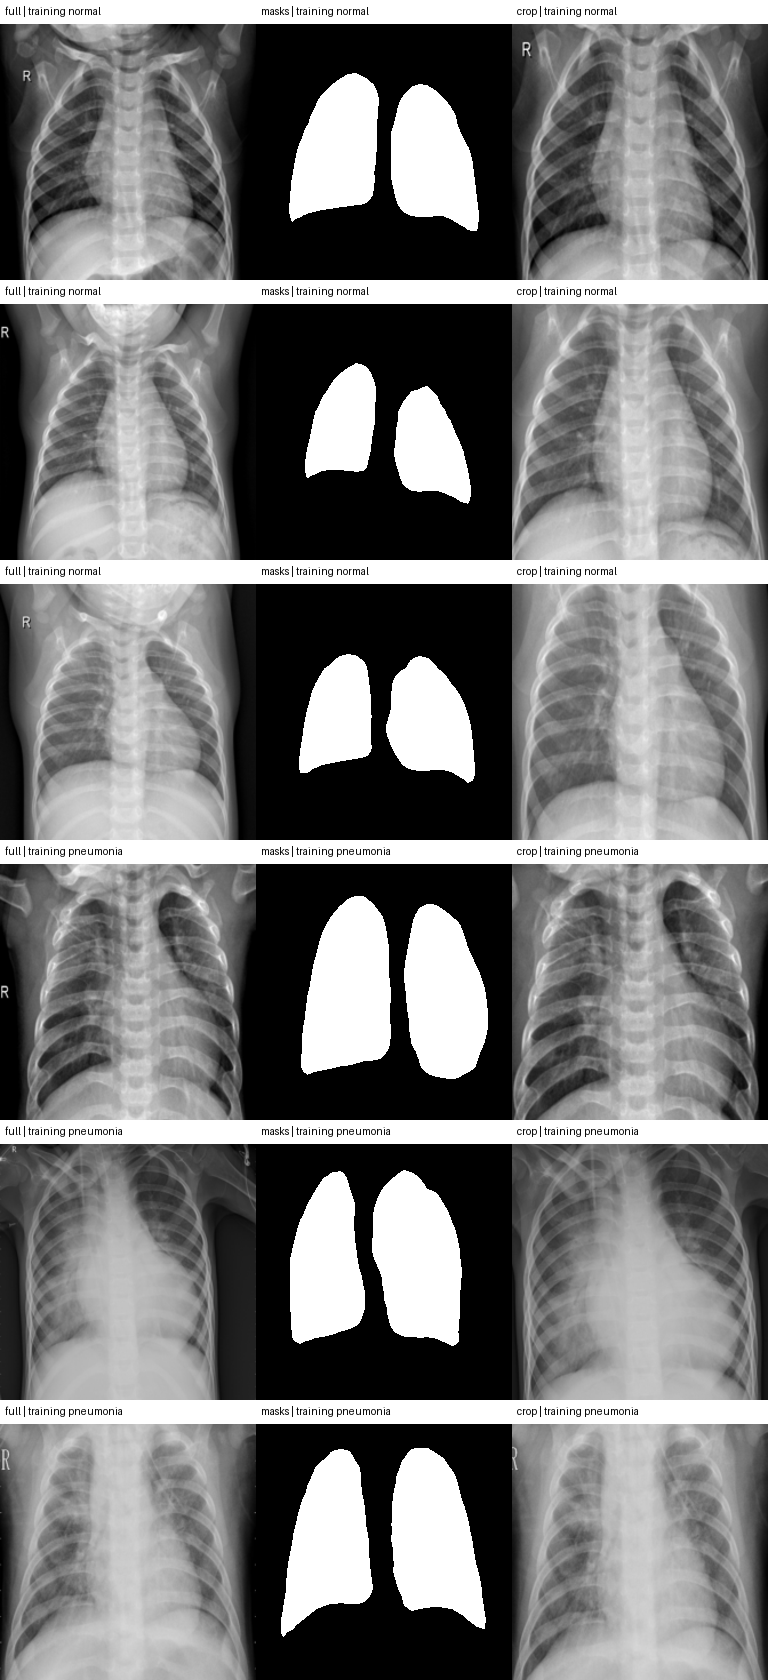
\includegraphics[width=.86\textwidth,height=.78\textheight,keepaspectratio]{training_balanced_mask_sanity.png}\caption{Predeclared training examples from both classes: full image, predicted mask and crop. These are qualitative outputs, not segmentation ground truth. Side markers may remain.}\end{figure}
\clearpage\section{Training History and Reproducibility}
\begin{figure}[!ht]\centering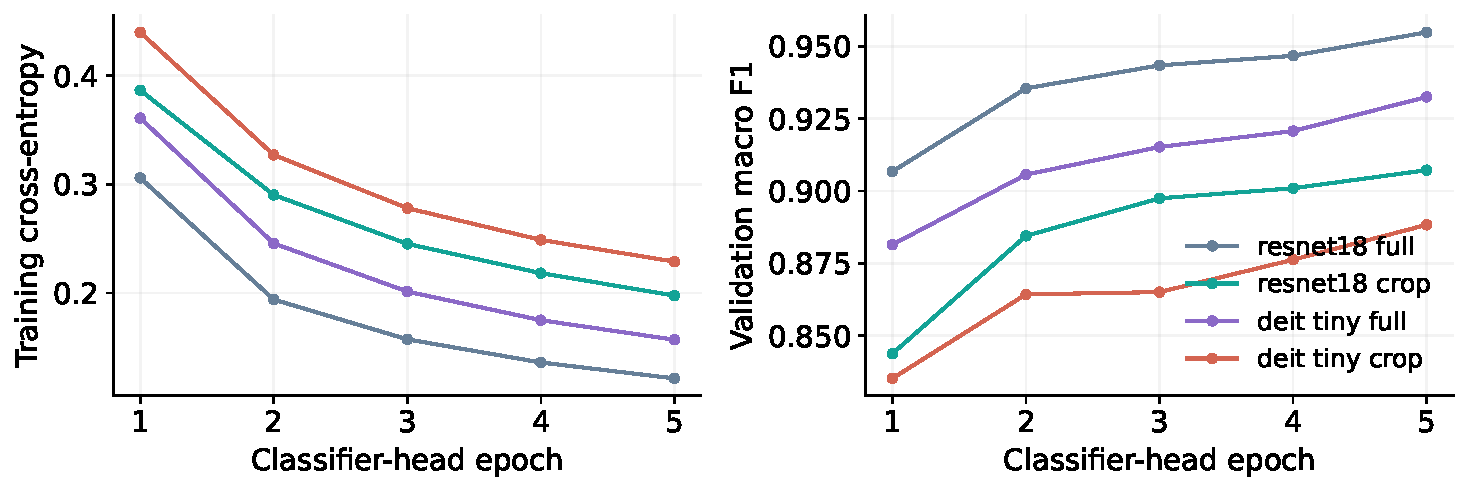
\includegraphics[width=.94\textwidth]{head_histories.pdf}\caption{Five-epoch histories for all four heads. Encoders remain frozen; all selected checkpoints are epoch five.}\end{figure}
\begin{figure}[!ht]\centering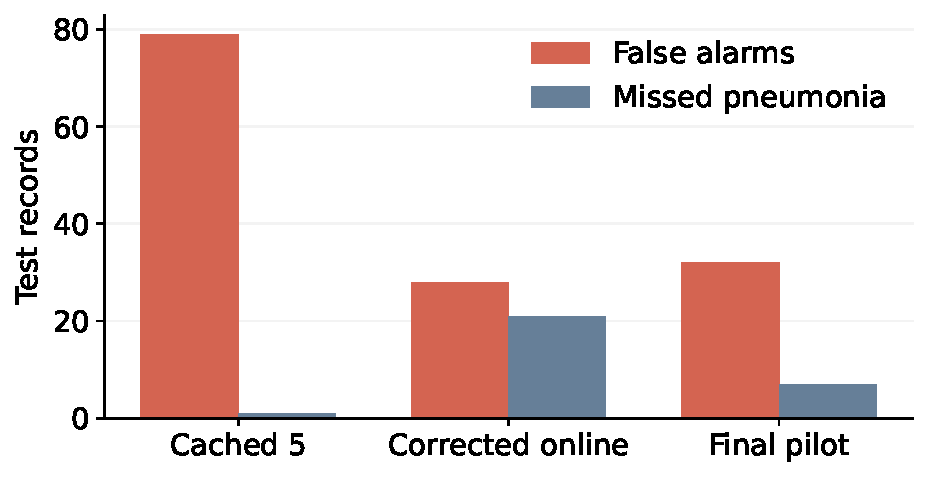
\includegraphics[width=.78\textwidth]{errors_history.pdf}\caption{Historical false-alarm and missed-case counts expose tradeoffs hidden by sensitivity alone. These are different protocols, not a causal ablation.}\end{figure}
\begin{table}[!h]\caption{Artifact verification summary.}\centering\begin{tabular}{ll}\toprule\rowcolor{RRlight}Check & Observed result\\\midrule
CSV metrics for A/B/C/D & Independently recomputed\\
Training-only feature scalers & Verified for all four heads\\
Validation checkpoint/weight selection & Recomputed from saved artifacts\\
Head replay on stored features & Maximum probability difference 0\\
Live model fixture replay & Difference approximately $3\times10^{-8}$ or less\\
Portable weights and inference & Network-disabled test passed\\
Model transfer integrity & All 21 manifest files matched\\\bottomrule\end{tabular}\end{table}
\clearpage\section{Selected Classification Errors}
\begin{figure}[!ht]\centering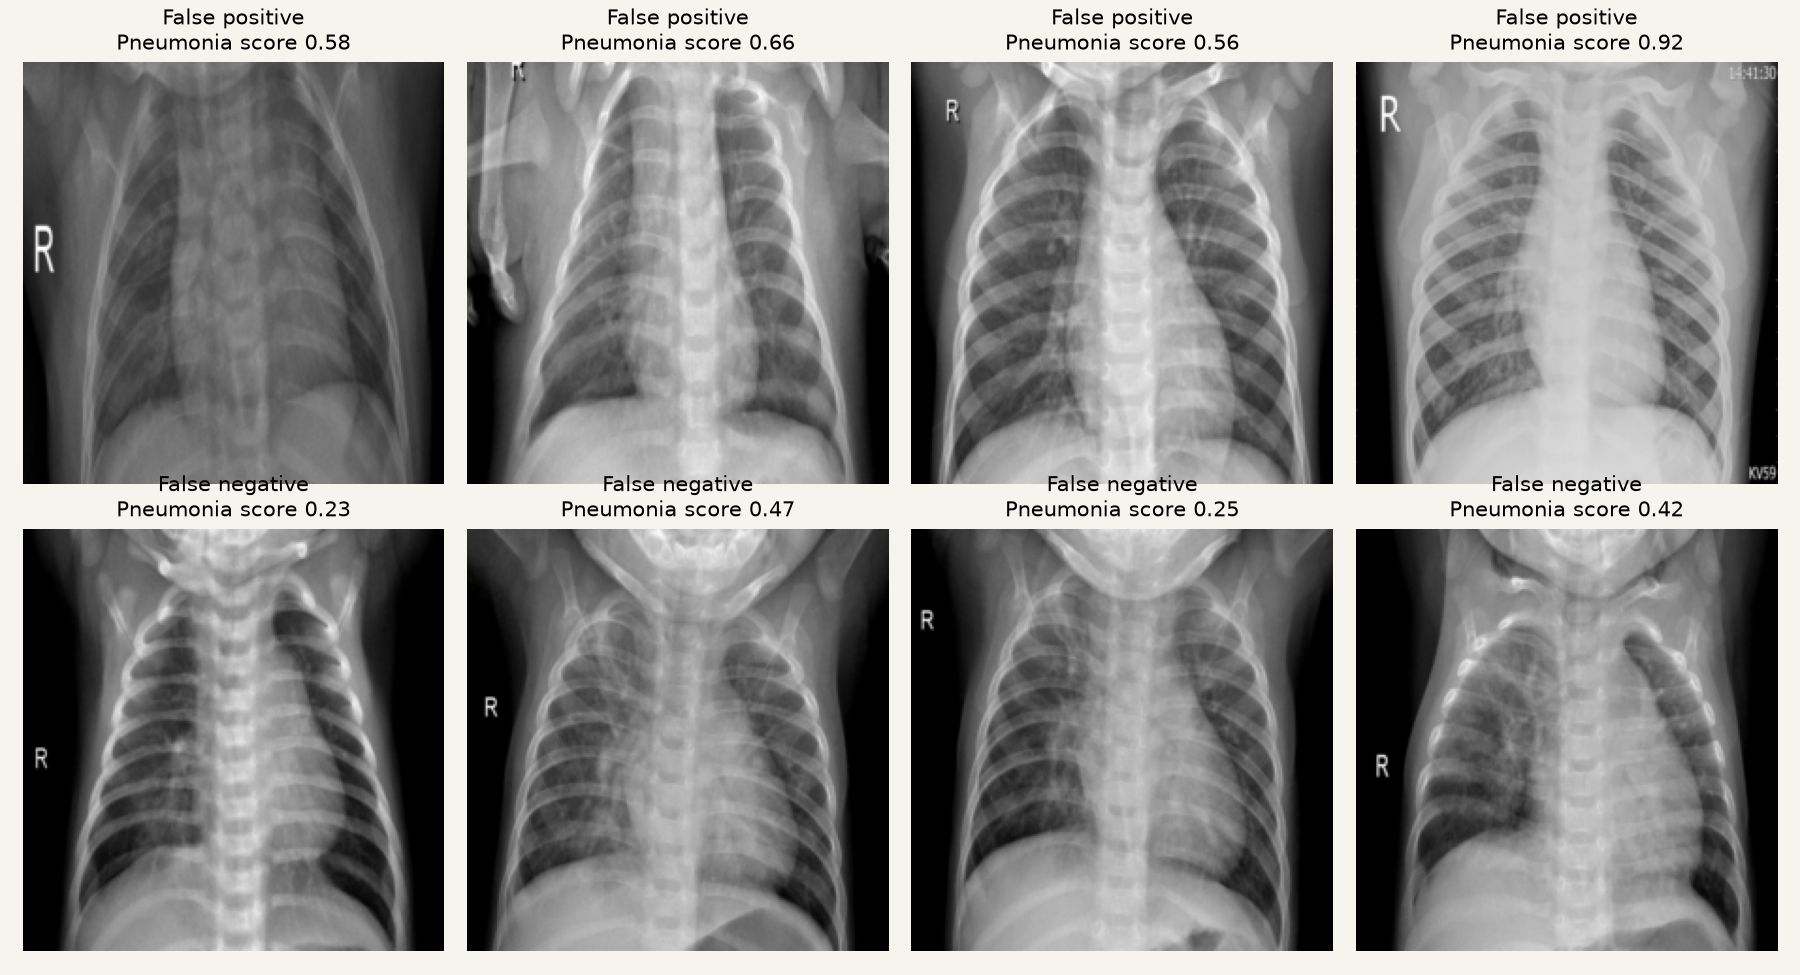
\includegraphics[width=.94\textwidth]{baseline_errors.png}\caption{Eight errors from the historical corrected M2 ensemble. These are actual benchmark records, not synthetic or selected correct predictions.}\end{figure}
\begin{figure}[!ht]\centering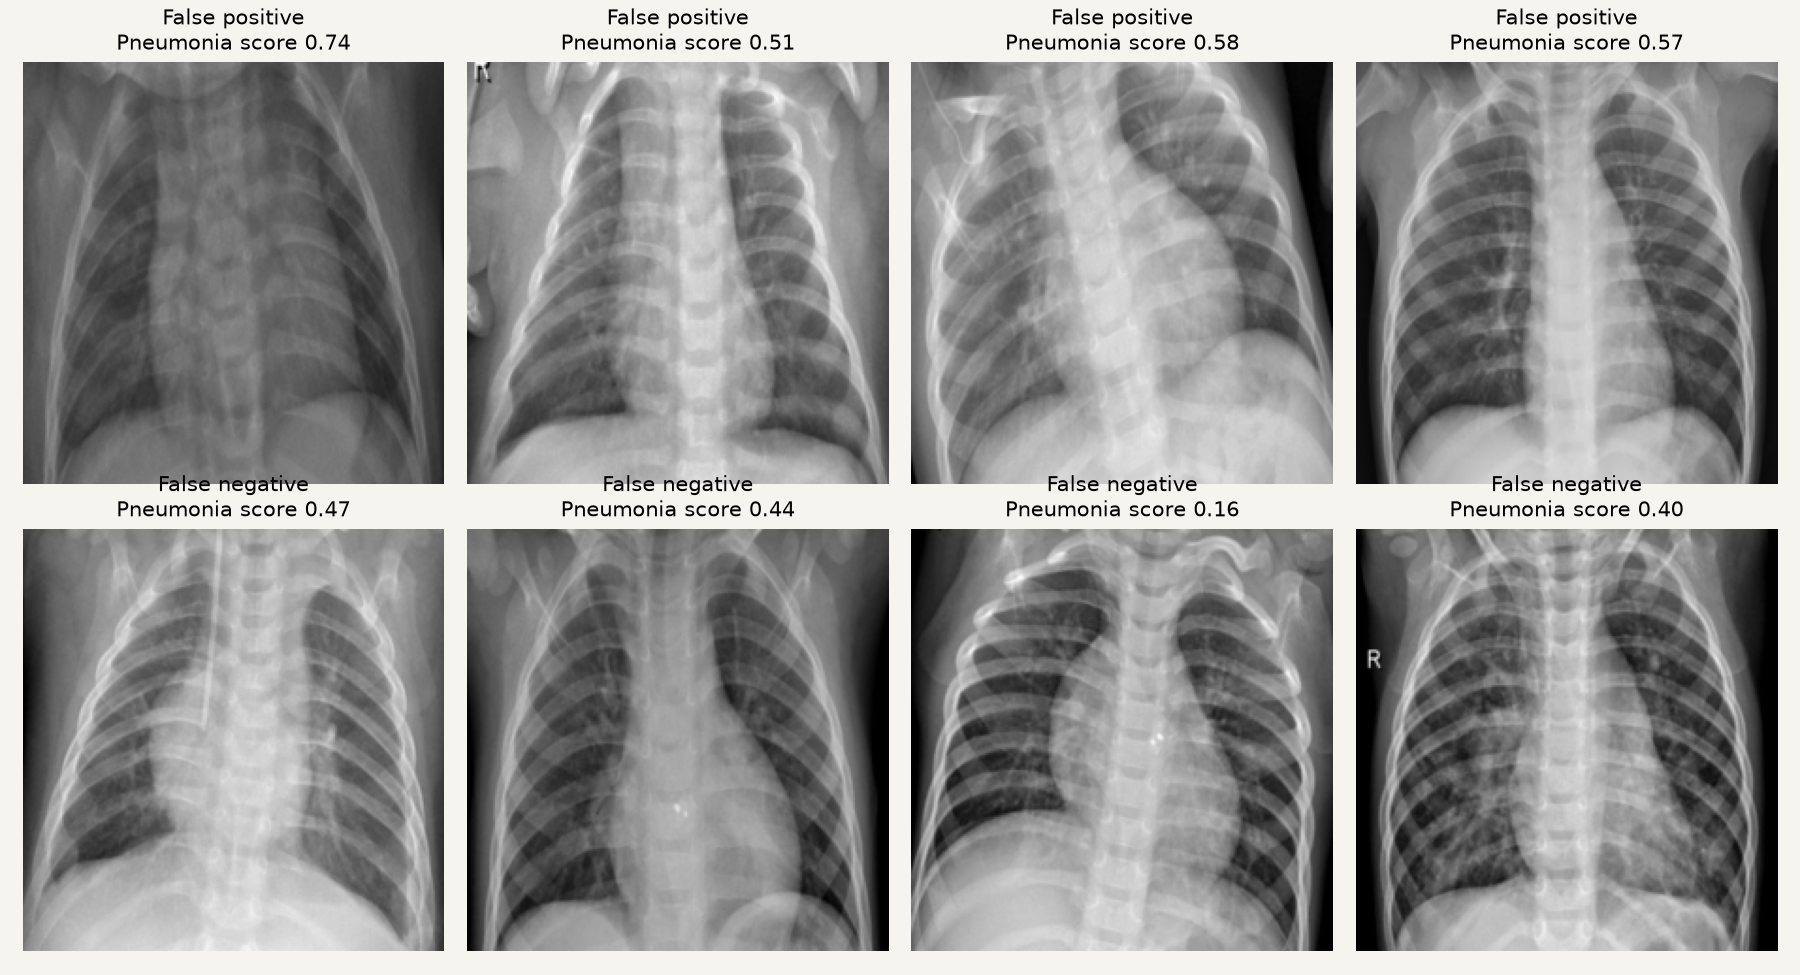
\includegraphics[width=.94\textwidth]{pilot_errors.png}\caption{Eight unique D errors: four false positives and four false negatives. Scores are uncalibrated pneumonia outputs, not medical certainty or adjudicated causes of error.}\end{figure}
\end{document}
